\documentclass[a4paper,11pt]{article}

\frenchspacing
%\usepackage[finnish]{babel}
%\usepackage[utf8x]{inputenc}
\usepackage{graphicx}
\graphicspath{{img/}}
\usepackage{tikz}
\usetikzlibrary{
  patterns,
  shapes.arrows, 
  shapes.geometric, 
  calc,
  fadings, 
  decorations.markings, 
  decorations.pathmorphing, 
  chains, 
  positioning, 
  intersections,
  snakes,
  spy,
  backgrounds,
  fit,
  arrows,
  automata,
  matrix}
\usepackage[americanresistors]{circuitikz}

%\usepackage[T1]{fontenc}
\usepackage{url}
\usepackage{cite}
%\usepackage{hyperref}
\usepackage{amsfonts,amssymb,amsbsy,amsmath,amsthm}
\usepackage{dirtree, array}
\usepackage{booktabs}
\usepackage{appendix}
\usepackage[ddmmyyyy]{datetime}

\usepackage{pgfplots}
\usepackage{pgfplotstable}
\usepgfplotslibrary{units}
\usepgfplotslibrary{groupplots}
\usepackage{floatrow}
\usepackage{subcaption}
\usepackage{multirow}
\usepackage{rotating}
\usepackage{algorithmic}
\usepackage{algorithm}
\usepackage{listings}
\usepackage{eqparbox}

\usepackage{siunitx}
\usepackage[pdfpagemode=UseNone,colorlinks=true,urlcolor=red,%
linkcolor=blue,citecolor=black,pdfstartview=FitH]{hyperref}
\usepackage[ddmmyyyy]{datetime}

\renewcommand{\dateseparator}{.}
%\usepackage[sorting=none]{biblatex}
\usepackage{placeins} % prevents the floats from passing a FloatBarrier
%% Define a new 'leo' style for the package that will use a smaller font.
\makeatletter
\def\url@leostyle{%
  \@ifundefined{selectfont}{\def\UrlFont{\sf}}{\def\UrlFont{\small\ttfamily}}}
\makeatother
%% Now actually use the newly defined style.
%\urlstyle{leo}
\begin{document}

\begin{titlepage}
\pagestyle{empty}
\begin{center}

\vspace*{3cm}
\noindent\LARGE{\textbf{
%
%*******************************************************
%Title:
Polygraph implementation using Arduino microcontroller board
%*******************************************************
%
}}
\\
\vspace*{1cm}
\large{
\begin{tabular}{l l}
%
%*******************************************************
%Author:
Henrik Lindblom & 67558R \\
Anne Vainio & 66535U \\
Aki Kauppinen & 12345A
%*******************************************************
%
\end{tabular}

\vspace*{1cm}
\begin{tabular}{l l}
Date & \textbf{
%
%*******************************************************
% Date
\today 
%*******************************************************
%
}
\end{tabular}
}
\end{center}
\end{titlepage}
%kansilehti loppuu 
\pagenumbering{roman}
\tableofcontents
\newpage
\pagenumbering{arabic}
%Varsinainan selkkari alkaa
\section{Introduction}
This paper describes the design and implementation of a polygraph,
more commonly referred as a \emph{lie detector}. The purpose of the
device is to determine whether a person, the \emph{subject}, is
telling the truth when asked simple yes or no questions, e.g. ``Have
you seen this man before?''. The polygraph measures the symphatetic
nerve activity of the subject through the electrodermal response, EDR,
combined with pulse and a video recording of the subjects facial
movements during the test. It is believed, but not implied by this
paper, that telling a deliberate lie induces a corresponding,
spontaneous response from the nervous system, which, when measured,
can be used to discriminate the questions where the subject is not
telling the truth. The basis for measuring the spontaneous response is
the EDR, which measures the sweat gland activity of the subject that
is known to correlate well with symphatetic nerve
activity\cite{Malmivuo1995}.
\begin{figure}[htb]  
  \caption{Block diagram of the device.}
  \label{fig:block-diagram}
  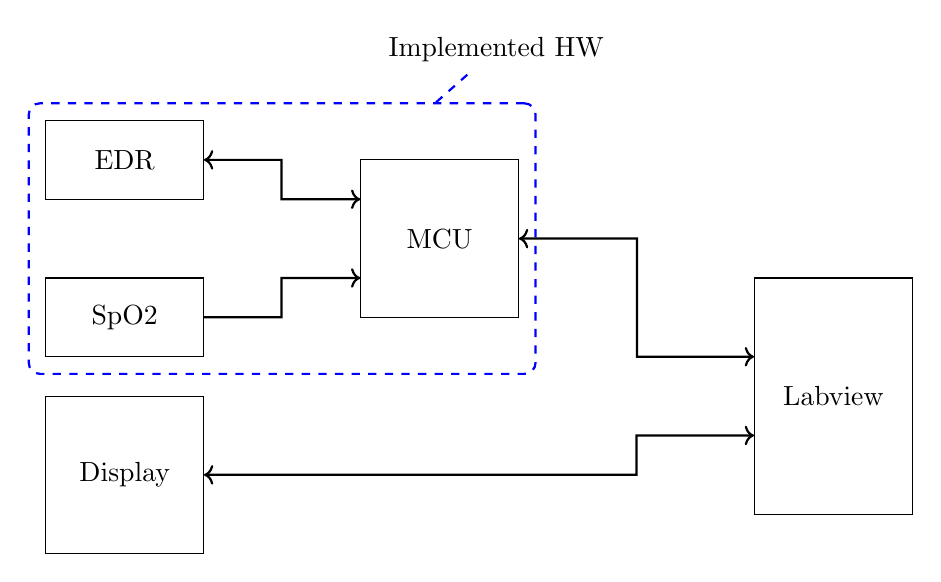
\begin{tikzpicture}[
      MCU/.style={
        minimum size=2cm
      },
      block/.style={
        rectangle,
        draw,
      },
      measurement/.style={
        minimum width=2cm,
        minimum height=1cm,
      },
      PC/.style={
        minimum height=3cm,
        minimum width= 2cm,
      },
      fitted-box/.style={
        draw=blue, 
        dashed, 
        rounded corners,
        inner sep=6pt,
        thick,
        rectangle,
      },
      display/.style={
        minimum height=2cm,
        minimum width=2cm,
      },
    ]
    \coordinate (mcu) at (0,3);
    \coordinate (pc) at (5,1);
    \coordinate (edr) at (-4,4);
    \coordinate (spo2) at (-4,2);
    \coordinate (touch-display) at (-4,0);
    \node[block, MCU] (mcu-node) at (mcu) {MCU};
    \node[block, PC]  (pc-node) at (pc) {Labview};
    \node[block, measurement] (edr-node) at (edr) {EDR};
    \node[block, measurement] (spo2-node) at (spo2) {SpO2};
    \node[block, display] (display-node) at (touch-display) {Display};
    \draw[<->, thick] (mcu-node.west) ++(0,0.5) -| ++(-1,0.5) -- (edr-node.east);
    \draw[<-, thick] (mcu-node.west) ++(0,-0.5) -| ++(-1,-0.5) -- (spo2-node.east);
    \node[fitted-box,fit=(mcu-node) (edr-node) (spo2-node), pin={[pin edge={blue, thick, dashed}]60:Implemented HW}] {};
%    \node[fitted-box,red, inner sep=10pt, fit=(edr-node) (spo2-node) (display-node)] {};
    \draw[<->, thick] (display-node.east) -| (2.5,0.5) -- ($(pc-node.west) + (0,-0.5)$);
    \draw[<->, thick] (mcu-node.east) -| ++(1.5,-1.5) -- ($(pc-node.west) + (0,0.5)$);
  \end{tikzpicture}
\end{figure}
The measurements are done using a microcontroller that converts the
analog signals to digital form and, additionally, communicates with a
host pc running a Labview software. The Labview softaware acts as a
graphical user interface, which displays and records the gathered
data. Furthermore, from the example question presented above it is
obvious that a method for displaying images for the subject is
required. The images must be synchronised with the questions in order
to reliably combine the measured response with a question. The images
are displayd to the subject using the same Labview software and an
additional touch screen display placed in front of the subject. A
block diagram of the device is presented in figure
\ref{fig:block-diagram}.

\section{The Electrodermal Response}
The skin consist of layers of alive and dead cells, called
\emph{epidermis}, \emph{dermis}, and \emph{hypodermis} with the
epidermis being the outer, and hypodermis being the inner layer of
skin. The layers protect the body from bacteria, mechanical assaults,
and dehydration and, in general, have a high electrical resistance;
the epidermis in particular is a strong electrical barrier. However,
since the body uses water to transfer excess heat from the body the
skin contains sweat glands and ducts that transfer sweat from the
hypodermis to the epidermis. The sweat glands are controlled by the
sympathetic nervous system, which implies two things. First, the
nervous system ensures that dehydration does not happen in excess and
water is excreted through the skin only during periods of elevated
body temperature or stress, such as heavy excercise or during a
humiliating situation. Second, sweating cannot be controlled by will;
a consequence of vast importance in the theory of
polygraphs.\cite{Malmivuo1995}

Sweat is a liquid with properties similar to a weak electrolyte. The
skin therefore consists of a number of parallel tubes filled with
conducting substance. When the sympathetic nervous system activates
the sweat glands, sweat is pumped through the outer layers of skin,
which result in a significant reduction in the skin resistance and,
consequently, the EDR measurement is an impedance measurement for
which several well known and tested circuit topologies exist. Like the
standard impedance measurement, the EDR has a high dynamic range; a
problem routinely encountered in regular multimeters. To counter this
problem, multimeters use a variable dynamic range to ensure sufficient
resolution even at extremely high impedances in the megaohm
range. Since the described method for solving the range problem is
routinely used by the industry, it is also the method chosen to
measure the electrodermal response.

Since the subject is a human being care must be taken not to cause any
pain or discomfort during the measurement. The impedance can be
measured either through the \emph{exosomatic} or \emph{endosomatic}
method. The first uses an external measurement current to cause a
voltage drop between two skin electrodes on the subject while the
other operates using the internal potentials of the
body\cite{Malmivuo1995}. The exosomatic method, while simpler, has the
potential to induce large enough currents in the body to induce
sensory stimulus, i.e. pain. In contrast, the endosomatic method
requires an amplifier with substantially higher input impedance than
the skin resistance, but does not drive a current through the
body.\cite{Malmivuo1995}

The skin measurement can be \emph{tonic} measuring the background
level of the impedance, or \emph{phasic} measuring the changes in the
signal filtering out any DC components. The suggested frequency range
for these measurements are typical for biosignal measurements:
\numrange{0}{5}\si{\hertz} for the tonic, and
\numrange{0.03}{5}\si{\hertz} for the phasic measurements.\cite{Malmivuo1995}
\begin{figure}[htb]
  \caption{A simplified qualitative equivalent circuit of the skin impedance between two electrodes.}
  \label{fig:edr-equivalent-circuit}
  \ctikzset{bipoles/length=0.8cm}
  \begin{circuitikz}
%    \node (corneum-resistance) at (
    \draw (0,1) to[battery, l=$E_1$] (0,0);
    \draw (0,1) to[R, l_=$R_4$] ++(0,1)
    to[R, l_=$R_2$] ++(0,1) node (epidermis-start) {} -- ++(0,1.7) 
    node (junction1) {} -- ++(1.7,0)
    to[R, l=$R_3$] ++(0,-1)
    to[battery,l=$E_1$] ++(0,-1) -- (1.7,0)
    ;
    \draw (junction1) to[R, l_=$R_1$] ++(0,1) -- ++(0,1.7) node (epidermis-end) {}
    -- ++(3,0) node[pos=0.5] (arrow-up) {} to[R,l=$R_5$] ++(0,-1) to[battery, l=$E_3$] ++(0,-1) -- (3,0)
    ;
    \draw (0,0) -- (3,0);
    \node (arrow-down) at (1.5, 0) {};
    \draw[<-] (arrow-down.center) |- (4.7,-0.5); 
    \draw (4.7,-0.5) -- (4.7,3.2) to[short, -o] ++(0.5,0) node (lower-terminal) {}
    ;
    \draw[<-] (arrow-up.center) |- (4.7,7.9);
    \draw (4.7,7.9) --(4.7,4.2) to[short, -o] ++(0.5,0) node (upper-terminal) {};
    \draw (upper-terminal) edge[bend left,->] node[pos=0.5, right] {}  (lower-terminal) ;
    \node[right] at (upper-terminal) {$+$};
    \node[right] at (lower-terminal) {$-$};
    \draw[
      thick,
      decoration={
        brace,
        raise=0.5cm,      
      },
      decorate
    ] (0,0) -- ({0,0}|-{epidermis-start.south}) 
        node[
          pos=0.5,
          xshift=-1.2cm,
          anchor=north, rotate=90] {Dermis};

    \draw[
      thick,
      decoration={
        brace,
        raise=0.5cm,
      },
      decorate
    ] ({0,0}|-{epidermis-start.north}) -- ({0,0}|-{epidermis-end}) 
        node[
          pos=0.5,
          xshift=-1.2cm,
          anchor=north, rotate=90] {Epidermis};



  \end{circuitikz}
\end{figure}
The simplified equivalent circuit of figure
\ref{fig:edr-equivalent-circuit} assumes lumped parameters, which may
or may not be appropriate for the distributed parameters of the
skin. Additionally, the model assumes that electrodes are used that
provide an efficient mechanism to convert between electron current
carriers inside the copper wires and the ions in the body. The
electrodes are placed firmly on the skin using a NaCl solution that
mimics the characteristics of sweat\cite{Malmivuo1995}.

Skin impedances decreases nearly exponentially with increasing
frequency, decreasing from \numrange{1}{3.5}\si{\mega\ohm} at
frequencies below \SI{10}{\hertz} to just \SI{220}{\ohm} at
\SI{1}{\mega\hertz}. However, the impedance is greatly lowered,
becoming nearly independent of frequency by removing the stratum
corneum, or the layers of dead cells in the epidermis, through
abrasion.\cite{Rosell1988} Other studies have found that skin
hydration increasingly affects the resistance of the measurement at
frequencies above \SI{100}{\kilo\hertz}\cite{Yamamoto1986}.

The recommended method for measuring electrodermal responses is to
measure the skin conductance, SC, using a approximately
\SI{0.5}{\volt} constant voltage source and a small series
resistor. The value of the series resistor should be chosen such that
the applied voltage between the two skin electrodes stays constant and
nearly \SI{0.5}{\volt}. In essence, the series resistor has to be
considerably smaller than the skin resistance, and a value of
\SI{500}{\ohm} has been recommended in literature.  Similar
recommendations have been made as per the electrodes used in the
measurement. The electrodes should be silver based, with Ag/AgCl being
a common choice, and they should be located on active sites with the
palmar side of hand being a particularly suitable place. In case of
skin potential measurements, the other electrode has to be placed in a
indifferent location near the elbow. The electrode surface area should
be approximately
\SI{1}{\cm^2}.\cite{Fowles1981,Rosell1988,Yamamoto1986,Malmivuo1995}
\section{Measurement Hardware}
The MCU used by the device is the Arduino Uno, which is an Atmega328
based prototyping board largely used by enthusiastist and academics
alike. The board contains some IO pins, 6 analog inputs with a 10-bit
ADC, and a usb-serial connection to the PC. The Arduino is programmed,
using an open source Arduino GUI, through the serial interface with
the help of a custom bootloader precompiled into the Atmega328. The
process is fairly straightforward and the board is quickly
operational. The software comes with a multitude of libraries for
device control and data acquisition and masks many of the tedious
tasks, such as register handling and interrupts traditionally
necessary for microcontroller programming. In addition to the simple
IO ports, some IO pins have an alternative function, namely the
hardware supported Universal Serial Interface (USI) capable of
communicating with peripheral devices using SPI. In the PC end, the
data is easily read into Labview, since a community maintained Arduino
library for communicating with the microcontroller exists and is
freely available through the VI Package Manager.
\subsection*{EDR}
As mentioned, the EDR is an impedance measurement with relatively high
dynamic range. Since the operator of the polygraph is interested in
the \emph{changes} in the signal, two possible implementations exist
that solve the dynamic range problem. First, the phasic measurement
can be used to disconnect any DC signals from the inputs of the
amplification circuit. Second, a variable gain amplifier can be used
to adjust the signal gain so that the signal is never clipped and
meaningful information can be read from the waveform. The latter
option can be implemented using, e.g. a digitally programmable
amplifier with an optional settable biasing voltage, generated for
example using a single channel DAC. The former option is easier to
implement, but exceedingly large capacitor values are needed to allow
the very low frequencies of the EDR to pass through the decoupling
capacitor. The second option is arguably more complicated and has many
more design parameters to be optimised, but the constraints on each
parameter are much more relaxed. 

The EDR signal is a fairly weak signal in the presense of a strong
common mode voltage. Since the signal amplitude is small, the overall
system gain has to be large, which requires that the common mode
signal is somehow attenuated before amplification. The DC common mode
signal is removed by AC coupling the amplifier inputs, effectively
removing the DC-component of the signal. To ensure that even slow,
gradual changes are measured, the decoupling capacitors must be
relatively large to position the -3dB frequency sufficiently low. An
appropriate value for the corner frequency should be < \SI{1}{\hertz},
and 0.3Hz was was chosen. Since the op amp inputs have negligible, but
non-zero, input bias currents a DC path must be provided from the
decoupled op amp inputs to ground. The easiest way to accomplish this
is to place a resistor between the input and ground.

Since EDR is concerned with the changes in the electrical properties
of skin, the measurement should be reasonably linear. Consequently, it
is convenient to measure the inverse of skin resistance, the skin
conductance $g_s$, which varies linearly when the sweat glands begin
to conduct. To measure the skin conductance, current through the skin
resistance has to be measured and to measure the current, a small
sense resistor has to be placed in series with the measurement voltage
and the skin conductance. This series resistance, $R_{sense}$, causes
a small nonlinearity in the measurement, but, provided that $R_{sense}
<< R_{skin}$, the effect is negligible. The basic measurement setup is
presented in figure \ref{fig:meas-setup}.
\begin{figure}[htb]  
  \caption{Conductance measurement}
  \label{fig:meas-setup}
  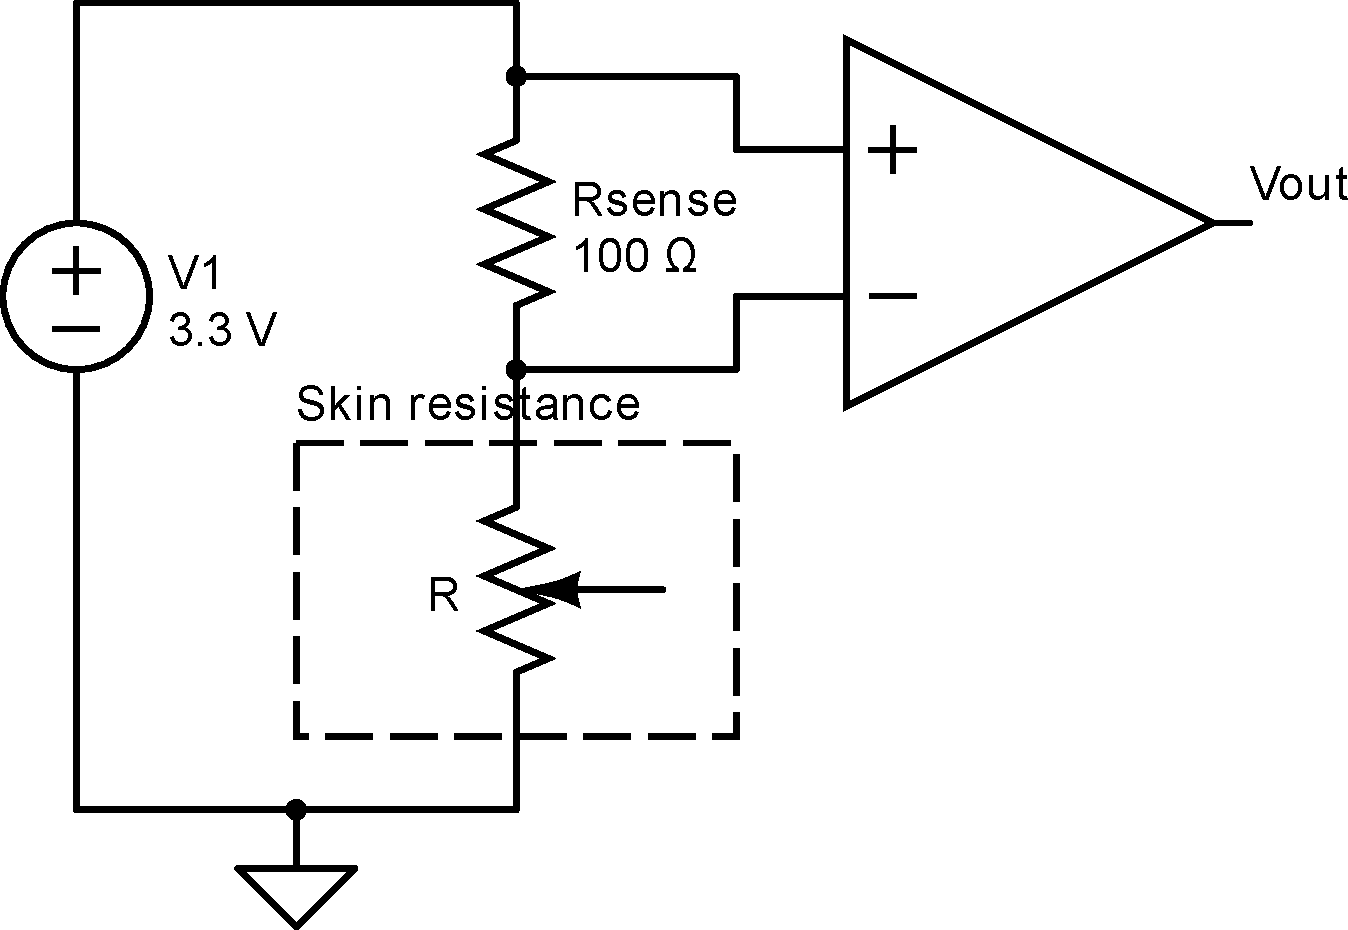
\includegraphics[width=\linewidth]{conductance_measurement}
\end{figure}

The output voltage of the setup presented in figure
\ref{fig:meas-setup} is $iGR_{sense}$, where $i$ is the current
through sense resistance and $GR_{sense}$ is the overall gain of the
amplifier. The current $i$ is calculated from the excitation voltage
as
\begin{equation}
  i = \frac{V_{meas}}{R_{skin} + R_{sense}} \approx \frac{V_{meas}}{R_{skin}} =
    g_sV_{meas},
\end{equation}
which is approximately linear in $g_s$. The overall gain of the system
determines the sensitivity of the measurement. The Atmega328 powering
the Arduino contains a 10-bit ADC with 5V reference voltage, setting
the minimum detectable voltage difference as $5/2^{10} \approx$
\SI{49}{\milli\volt}. Therefore, the necessary gain can be calculated
from 
\begin{align}
  G &= \frac{\SI{49}{\milli\volt}}{R_{sense}V_{meas} \Delta g_s},
\end{align}
where $\Delta g_s$ is the smallest measrurable change in
conductance. However, if the smallest measurable conductance is fixed
to an absolute value, the \emph{dynamic range} of the amplifier has to
be fairly large since a \SI{1}{\kilo\ohm} change is roughly 10\% in
the 10k range but only 0.1\% in the mega Ohm range. Therefore, the
required sensitivity is defined as the smallest measurable relative
change, and given as a percentage.

Since the total required gain is quite high, the gain block has to be
divided into several blocks with reasonable gains to prevent the
amplifier stage from becoming unstable. Amplifiers with very high
gains might start to oscillate if, at some frequency, the gain has
reduced to unity and the phase of the signal has turned
\SI{180}{\degree}, i.e. inverted, resulting in positive feedback which
quickly saturates the output. To prevent this, stages with lower gain
are used in series to achieve the same required total gain. Since the
desired signal, changes in the skin conductivity, is measured across
the sensing resistor $R_{sense}$ in the precence of a large common
mode DC-voltage. As instrumentation amplifiers have, in general, much
larger common mode rejection ratios than ordinary operational
amplifiers, the first amplifier stage was built using the AD8236
instrumentation amplifier, which has adjustable gain from 5 to 200
using only one external resistor. The AD8236 has a reference terminal
to which the output voltage is referenced. By capacitively coupling
the input of the amplifier back to the reference terminal, the gain of
the amplifier is reduced to unity at low frequencies while remaining
high at higher frequencies, effectively AC coupling the amplifier. The
AC coupled instrumentation amplifier circuit topology is presented in
figure \ref{fig:ina-ac-coupled}.
\begin{figure}[htb]   
  \caption{AC coupled AD8236. Schematic taken from the datasheet.}
  \label{fig:ina-ac-coupled}
  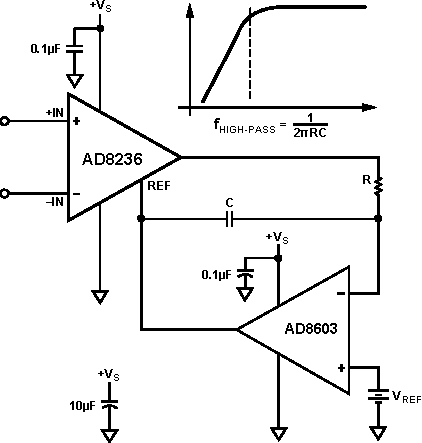
\includegraphics[width=\linewidth]{ina-ac-coupled}
\end{figure}
The voltage Vref shifts the output of the amplifier to the middle of
the available voltage range, providin Vs/2 volts of swing room for the
varying EDR signal. The op amp selected as the buffer for the REF pin
was chosen to be the same as recommended by the datasheet.

The second amplifier stage is also AC coupled to prevent the virtual
ground at Vs/2 from being amplified thus saturating the output. Since
the reference pin is buffered by a AD806, it is logical to choose the
same amplifier as the second amplifier stage since the op amp comes in
single, dual, and quad configurations, which is convenient and saves
board space. The second AD806 is connected as a AC-coupled,
non-inverting amplifier that is biased at Vs/2 to provide the same
head room for the AC signal as the first stage. The biasing is done by
simply forming a voltage divider at the positive input terminal. The
voltage divider also serves as a DC return path to ground, preventing
the input bias currents of the amplifier from generating a DC voltage
to between the inputs. The gain of the amplifier is initially chosen
as 36, but should this be inadequate, the gain can be safely increased
by adjusting the feedback resistors.

The final amplifier stage is a programmable amplifier with user
selectable gains from 1 to 16, and is intended for fine tuning the
signal amplitude before the ADC inputs. The gain is initially set to
the middle of the gain range, i.e. 8, and can then be altered via the
microcontrollers SPI interface. This configuration can then be used to
either double or halve the gain if the signal amplitude is too weak or
too large respectively. The amplifier initially chosen for this task
was the TI LMP8100, as the supply of SPI controllable amplifiers
seemed somewhat scarce, which was a fallacy since there actually
exists a wide range of different programmable amplifier devices. 
\begin{figure}[htb]   
  \caption{AC coupled non-inverting amplifier}
  \label{fig:ac-coupled-non-inverting}
  \includegraphics[width=0.7\linewidth]{ac-coupled-non-inverting}
\end{figure}
One alternative would have been a regular op amp with a digitally
controllable feedback resistor network. This would have had the
advantage that the gains could be easily selected and adjusted, but on
the other hand, the configuration would have taken much more board
space than a single programmable device. The DIY option could have
been implemented with the help of a analog switch and the output pins
of the Arduino mini, optionally using a parallel out shift register,
such as the 74HC595, to reduce the output pin usage.

\subsection*{Pulse}
Pulse is measured using a Medlab pulse oximetry module EG00352, which
connects to a SPO2 led sensor, measures the amount of light absorbed
by oxygen in the blood, and calculates the oxygen saturation and pulse
of the patient. The signals are continuously transmitted over a serial
transmit wire operating at CMOS logic levels, i.e. from 0 to 3.3V, with a baudrate of
9600. The module requires only a well regulated 3.3V supply and ground
signals, as well as connections to the SPO2 sensor leads; it is
otherwise self contained.

The required 3.3V is generated from the 5V usb lead with the help of a
LM317 voltage regulator. The LM317 is a three terminal positive
adjustable voltage regulater, with output voltage selectable using two
external resistors. The device operates by maintaining a fixed
\SI{1.25}{\volt} voltage between the OUT and GND, also commonly
referred to as ADJ, terminals. The regulator circuit is presented in
figure \ref{fig:3V-reg}. The output voltage is given by
\begin{equation}
  V_o = 1.25\left(1+\frac{R_2}{R_1}\right) + I_{gnd}R_2,
\end{equation}
where $I_{gnd}$ is typically less than \SI{100}{\micro\volt} and can
be neglected for most applications. The equation follows from the fact
that current $I_1 = \frac{\SI{1.25}{\volt}}{R_1}$ flows into the GND-terminal
node, and since $I_{gnd}$ is small, the voltage from the output
terminal is $1.25V + I_1R2 = 1.25(1+\frac{R_2}{R_1})$.
\begin{figure}[htb]   
  \caption{\SI{3.3}{\volt} voltage regulator.}
  \label{fig:3V-reg}
  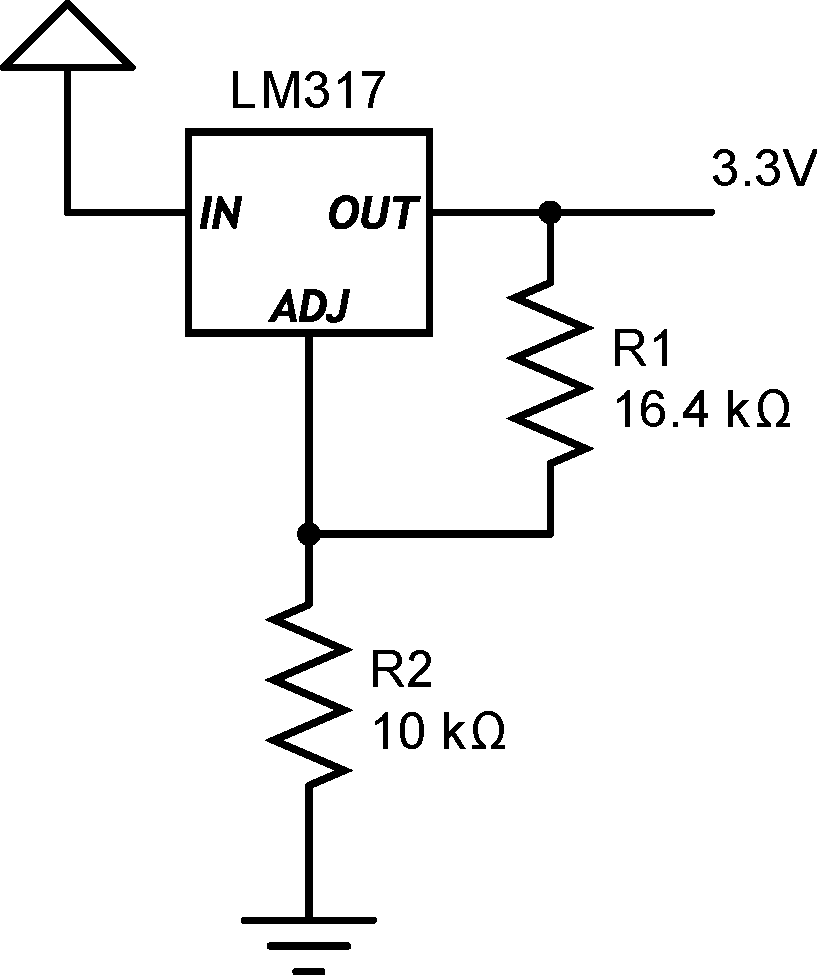
\includegraphics[width=0.5\linewidth]{3v-regulator}
\end{figure}

The serial data from the SPO2 module has to be
translated to TTL logic, i.e. from 0 to 5V, before it can be connected
to the Arduino. This is achieved by driving the gate of an NPN MOSFET
circuit presented in figure \ref{fig:logic-level-translation}. The
MOSFETs buffer the serial signal and cause the voltage at the serial
input to swing from GND to 5V, sufficiently for the Arduino to
register each bit.
\begin{figure}[htb]  
  \caption{Logic level translation. When Vin is HIGH Q1 is conducting
    and the gate of Q2 is pulled close to ground, causing Vout to be
    pulled HIGH. When Vin is pulled low, Q1 closes and the gate of Q2
    is set to Vcc thus opening the DS-channel and pulling Vout to
    ground.}
  \label{fig:logic-level-translation}
  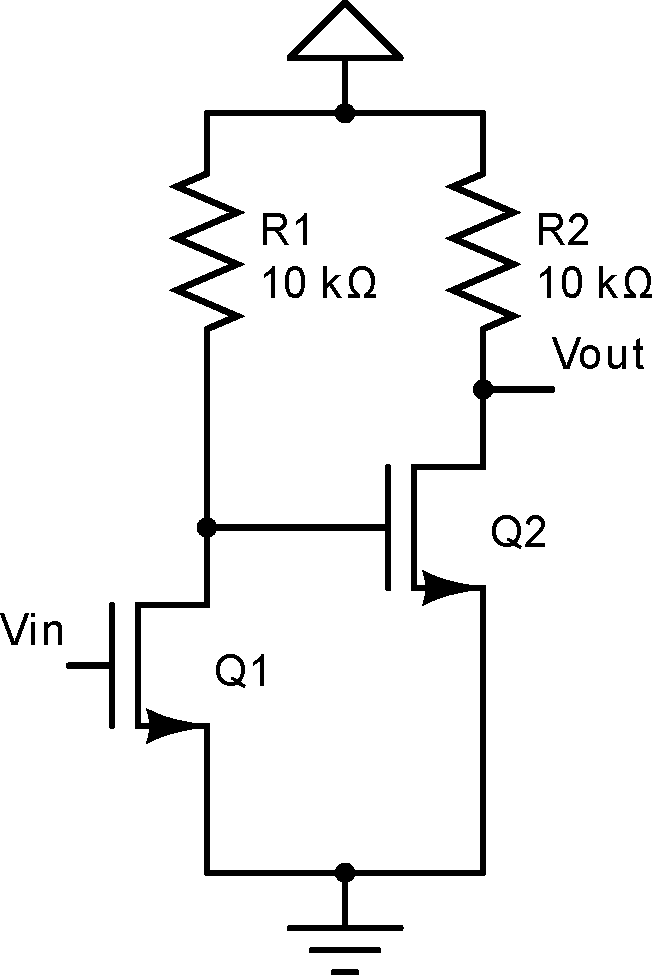
\includegraphics[width=0.5\linewidth]{level_converter}
\end{figure}

Since the main RX/TX pins of the Arduino are required for
communicating with the host computer, the SPO2 data is read using a
software serial library available for Arduino. The library assigns
external interrupts for each registered IO-pin and when the pin state
changes the software reads the current pin state directly from the
pin, essentially transforming any IO-port to a serial interface,
provided that the baud rate for communications is sufficiently low.
The baud rate of the Medlab module is, as mentioned, 9600, which a
relatively slow communication speed and should pose no problems to the
software serial implementation.

\section{Host Software}
The polygraph device sends data, and is controlled by the host
computer running a Labview program, which displays the questions to
the subjects and records the response. The Arduino is loaded with the
Labview Arduino interface firmware, which can be acquired through the
VI Package Manager. The library also provides many usefull subVIs for
control and data acquisition from the ADC. The program consists of an
user interface and a data acquisition loop that continuously collects
data from the Arduino. The UI and main loop are implemented using the
Labview event structure, which can be registered to wait for an user
interface event and has an inbuilt timeout event, which is fired if no
UI events occur before the preset timeout value, given in
milliseconds. The timeout event is practical for acquiring data, since
the code is fired at roughly equal intervals, and the event structure
is superior in monitoring the UI for actions, since no polling is
required for any of the front panel controls.

The questions are displayd to the subject through a subVI that is
launched on a separate window. The subVI takes two Labview queue
references as parameters and uses these to communicate to the main
application. Similarly, when the main application wishes to send data
to the remote application it simply puts the data in the send queue
and Labview core handles the rest. The subVI showing the questions is
operated using a touch screen, and consists of a large area for
displaying pictures and text and two boolean buttons for \emph{yes}
and \emph{no} answers.

\section{PCB Assembly}
The PCB was designed using the freeware version of CadSoft Eagle PCB
layout software. Some of the parts were directly available in the
various libraries, but the majority of the footprints had to be made
by hande, or acquired from external libraries. Particularly good 3rd
party libraries were found from www.sparkfun.com and www.lement14.com.
Since majority of components manufactured today come in surface mount
packages, and some of the components were only available in SMD
packages, no effort was made to search for alternative devices that do
come in through hole packages. The Medlab SPO2 module and Arduino are
attached to the PCB using pin headers, which allow the modules to be
removed if the device ever becomes obsolete, or if another improved
version is made. The SPO2 module connects to a low profile 2x4 and 2x3
(rox x col) male pin headers using 2mm pitch. The only suitable
manufacturer was found to be Samtec, but the somewhat expensive
headers were sold in batches of 10, making the headers one of the most
expensive parts in the assembled device. Luckily, two 2x5 Samtec low
profile headers were found lying around in a junk box and, although
larger than required, have much better price/functionality ratio than
the expensive headers of the right size. The price of each component
was assessed critically since the intended use of the device is not
precision resistance measurement but to give qualitative information
about the subconscious reactions of a subject being asked questions.

The freeware version of Eagle is capable of producing two layer PCBs
with size restrictions, but since much of the electronics were
separately packaged in the SPO2 and Arduino modules, all the
components were easily placed on the top layer, while the bottom layer
holds mainly the ground plane and a few signals. No particular high
speed design considerations were made in the design as the signals
being measured are relatively slow biosignals. EMC was also considered
as a non-issue since the intended use site of the device should not
contain possibilities for capacitively coupled fields in the
measurement frequency range since the pass band of the device
terminates before the \SI{50}{\hertz} power line frequency.

If this were a medical device, the patient would have to be isolated
from the main power supply. Murata, for example, makes handy power
isolators, but their price in small batches is unreasonably high, in
tens of euros, for this application. Another possibility would have
been the use of a transformer coil and a switching circuit generating
the required AC signal that would induce voltage in the secondary
coil. This approach however requires, in addition to the transformer
coils, a switching IC, a rectifier bridge on the isolated side as well
as a voltage regulator. Provided the component sizes were kept
reasonable to enable easy hand soldering, this would require board
space, but would improve the safety of the device. However, since the
probe leads connected to the subject are placed in adjacent fingers,
and since the \SI{100}{\ohm} sensing resistor limits the maximum
\emph{theoretical} current to \SI{33}{\milli\ampere}, which is not
sufficient to cause skin burns, the isolation was considered, but
ultimately left out of the apparatus.
%\subsection*{Video}

%% \nameref{section:UI} which actually handles the error. The user event data
%% \pagebreak
%% \begin{equation}
%%   e \propto ||\nabla T|| \propto \frac{\partial T}{\partial t}.
%% \end{equation}
%% The proportionality coefficients are calculated using the linear
%% regression model
%% \begin{align}
%%   \mbox{MEAS} &= \alpha_1T_1 + \alpha_2\frac{\partial T_1}{\partial t} +
%%   \alpha_0 \\
%%   \mbox{REF} &= \beta_1T_2 + \beta_2\frac{\partial T_2}{\partial t} + \beta_0
%% \end{align}
%% \begin{align}
%%   \mbox{MEAS}_{comp} &= \mbox{MEAS} - \alpha_1T_1
%%   -\alpha_2\frac{\partial T_1}{\partial t} \\
%%   \mbox{REF}_{comp} &= \mbox{REF} - \beta_1T_2 - \beta_2\frac{\partial T_2}{\partial t}.
%% \end{align}

%% \subsubsection{Time derivative}
%% \begin{figure}[htb]
%%   \includegraphics[width=\textwidth]{dataflow}
%%   \caption{Program dataflow chart. Arrows indicate direction of data flow,
%%     not dependance or sequentiality.}
%%   \label{fig:dataflow}
%% \end{figure}

%% \begin{figure}[htb]
%%   \includegraphics[width=\textwidth]{block-diagram-map}
%%   \caption{Block diagram functional components}
%%   \label{fig:block-diag-map}
%% \end{figure}

%Kirjallisuuviitteet
\bibliography{Polygraph}
\bibliographystyle{ieeetrans}

%% \appendix
%% \appendixpage
%% \addappheadtotoc
%% \section{Directory listing}

%% \begin{tabular}{l l}
%% %% \hline
%% %% \multicolumn{1}{c} {Heading 1} & \multicolumn{1}{c} {Heading 2} \\
%% %\hline
%% \begin{minipage}{0.3\linewidth}\dirtree{%
%% .1 mims-project.
%% .2 data. 
%% .2 docs. 
%% .2 helpers. 
%% .2 test. 
%% .2 typedefs. 
%% .2 utilities. 
%% .2 main.vi. 
%% }\end{minipage}
%% &
%% \DTsetlength{0pt}{0pt}{0pt}{0pt}{0pt}
%% \begin{minipage}{0.7\linewidth}\dirtree{%
%% .1 Root directory.
%% .2 Contains sensor-configurations.ini.
%% .2 Documents related to the sensor hardware.
%% .2 Some helpfull functions.
%% .2 Unit \& other tests.
%% .2 Controls and clusters used by the program.
%% .2 Functions for performing more complex tasks.
%% .2 The main program.
%% }\end{minipage}
%% \\
%% %\hline
%% \end{tabular}

\end{document}
